\documentclass[tikz, margin=3.14mm]{standalone}

\usepackage{tikz}
\usetikzlibrary{patterns, snakes, backgrounds}

\begin{document}
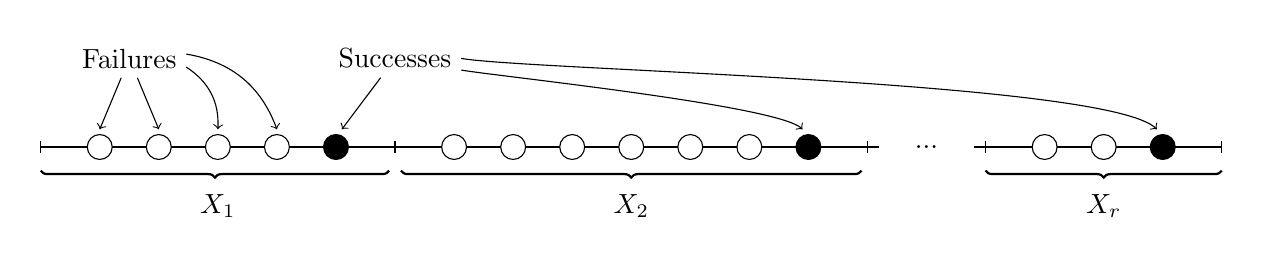
\begin{tikzpicture}[scale=1.5, background rectangle/.style={fill=white}, show background rectangle,]

\path (0,0) edge (7.1,0); % main numberline part 1
\path (7.9,0) edge (10,0); % main numberline part 2
\node at (7.5,0) {...};

\foreach \x in {0, 3, 7, 8, 10} {
\path (\x,-.05) edge (\x,.05);
}

% failures:
\foreach \x in {.5, 1, 1.5, 2, 3.5, 4, 4.5, 5, 5.5, 6, 8.5, 9} {
\filldraw [fill=white] (\x,0) circle (3pt);
}

% successes
\foreach \x in {2.5, 6.5, 9.5} {
\filldraw (\x,0) circle (3pt);
}

\draw[thick,decoration = {brace, mirror}, decorate] (0,-.2) -- (2.95,-.2);
\node at (1.5, -.5) {$X_1$};

\draw[thick,decoration = {brace, mirror}, decorate] (3.05,-.2) -- (6.95,-.2);
\node at (5, -.5) {$X_2$};

\draw[thick,decoration = {brace, mirror}, decorate] (8,-.2) -- (10,-.2);
\node at (9, -.5) {$X_r$};

\node (F) at (.75, .75) {Failures};
\path [->] (F) edge [bend left] (2,.15);
\path [->] (F) edge [bend left] (1.5,.15);
\path [->] (F) edge (1,.15);
\path [->] (F) edge (.5,.15);
\node (S) at (3, .75) {Successes};
\path [->] (S) edge (2.55, .15);
\path [->] (S) edge [looseness = .25, out = -10, in=135](6.45, .15);
\path [->] (S.east) edge [looseness = .25, out = -10, in=135] (9.45, .15);

\end{tikzpicture}
\end{document}